\documentclass{article}

\usepackage{fullpage}
\usepackage[colorlinks=true]{hyperref}
\usepackage[tableposition=top]{caption}
\usepackage[utf8]{inputenc}

\usepackage{Sweave}
\begin{document}
\Sconcordance{concordance:2016-01-21_MitochondrialProteins.tex:2016-01-21_MitochondrialProteins.Rnw:%
1 7 1 1 0 10 1 1 17 2 1 1 44 1 35 4 1 1 14 1 3 6 1 1 14 1 3 6 1 1 14 1 %
3 6 1 1 14 1 3 6 1 1 14 1 3 6 1 1 14 1 3 6 1 1 53 1 2 5 1 1 2 11 0 1 2 %
2 1}


\title{Analysis of Mitochondrial OXPHOS protein Levels in the Quadriceps from Gestationally Treated MCP230 Mice on a High Fat Diet}
\author{Erin Stephenson}
\date{2016-01-21}
\maketitle

\section*{Details}
{Protein lysates were prepared using standard protocols and quantified via Bradford assay. Equal protein was loaded into 2x 12 well gradient gels. Proteins were separated by SDS-PAGE and transferred to Nitrocellulose membranes. Membranes were blotted using the mitochondrial OXPHOS antibody cocktail from ABCAM. Protein content was determined from fluorescent images obtained on a LiCor Odyssey and quantified using Image Studio Lite software. Protein expression was normalized to total AMPK expression -which was not different between groups- and is presented here relative to the saline control group}
\section*{Data analysis}

The data is saved in \verb+C:/Users/esteph16/Documents/GitHub/ObesityParticulateTreatment/scripts/MitoProteinAnalysis+.  The raw data file for the first run is named \verb+PostReviewMitoWesterns.xlsx+.  

\section*{Statistics}
\section*{Figures}


\begin{figure}
\begin{center}
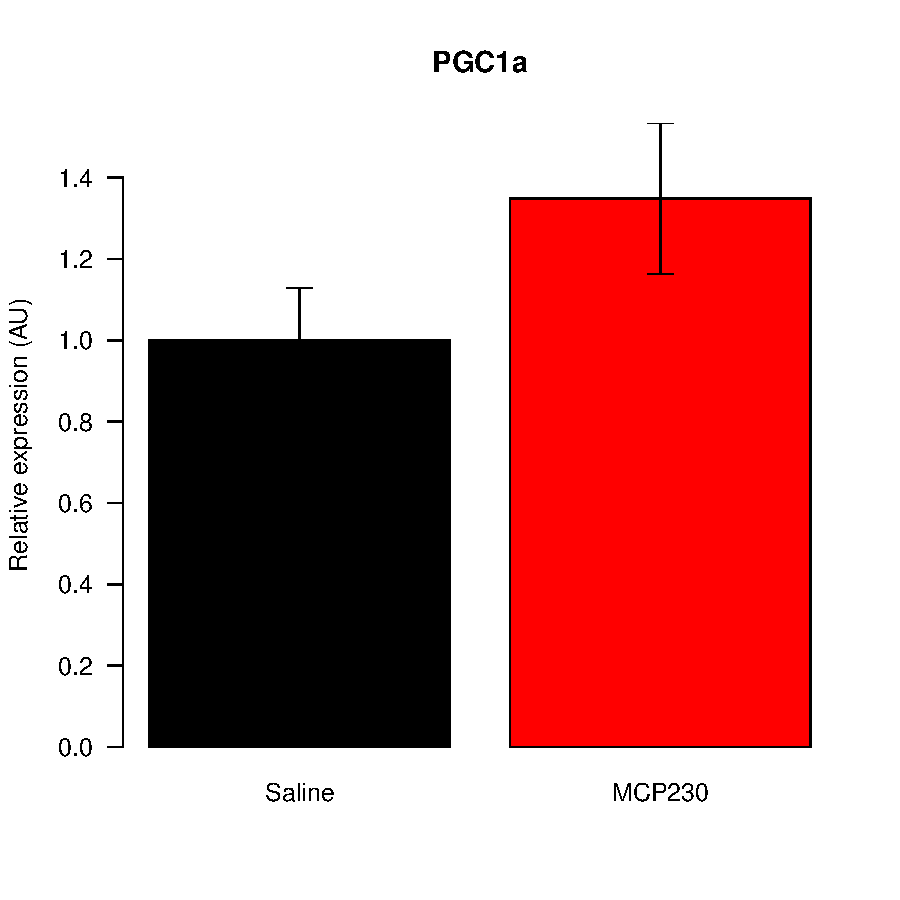
\includegraphics{2016-01-21_MitochondrialProteins-barplotPGC1a}
\end{center}
\caption{Barplot of Relative PGC1a Protein Expression in Quadriceps Muscle, Saline versus MPI}
\label{fig:barplotPGC1a}
\end{figure}

\begin{figure}
\begin{center}
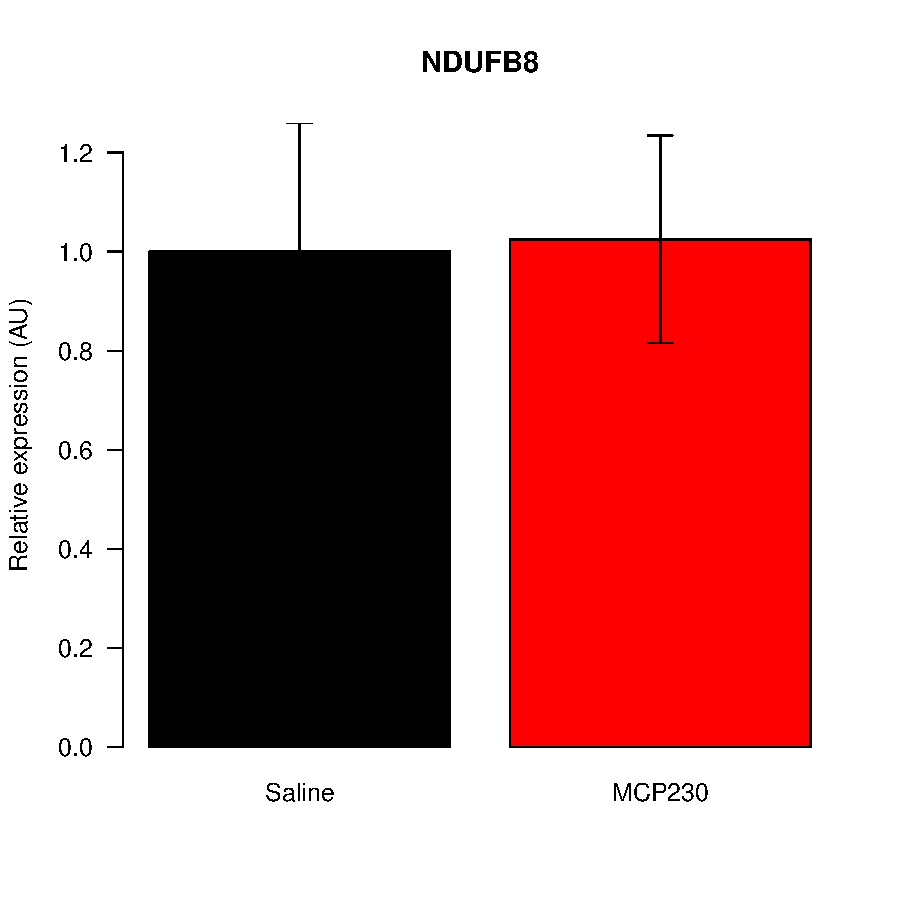
\includegraphics{2016-01-21_MitochondrialProteins-barplotNDUFB8}
\end{center}
\caption{Barplot of Relative NDUFB8 Protein Expression in Quadriceps Muscle, Saline versus MPI}
\label{fig:barplotNDUFB8}
\end{figure}

\begin{figure}
\begin{center}
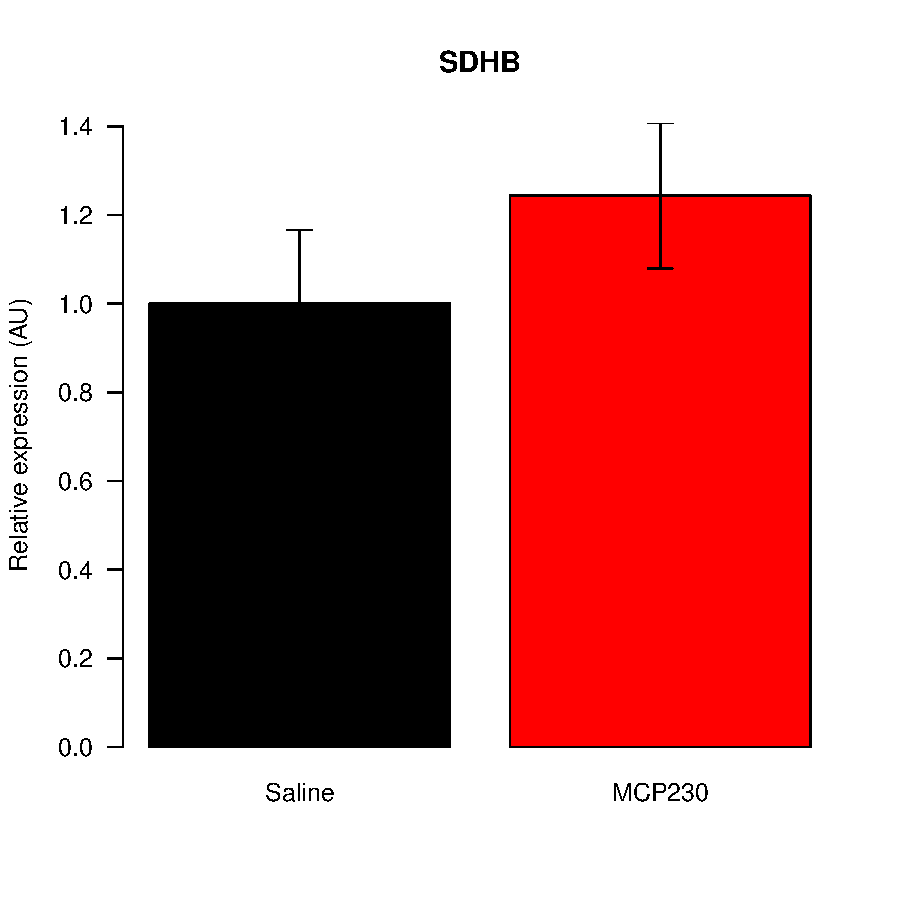
\includegraphics{2016-01-21_MitochondrialProteins-barplotSDHB}
\end{center}
\caption{Barplot of Relative SDHB Protein Expression in Quadriceps Muscle, Saline versus MPI}
\label{fig:barplotSDHB}
\end{figure}

\begin{figure}
\begin{center}
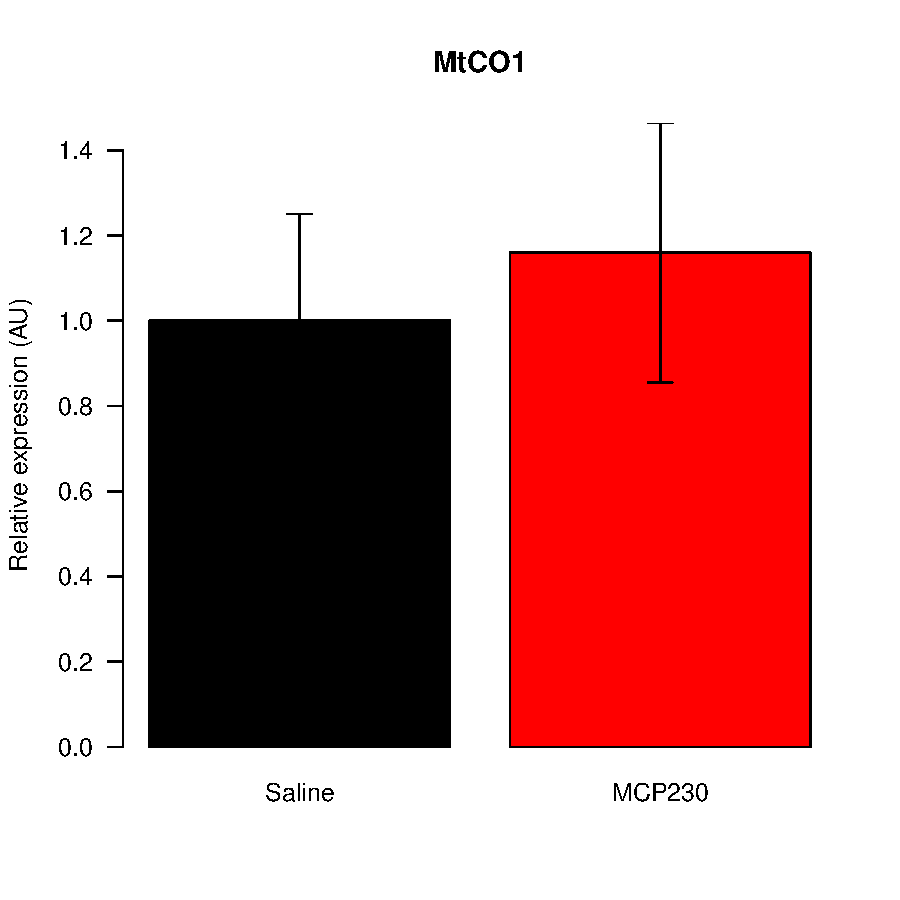
\includegraphics{2016-01-21_MitochondrialProteins-barplotMtCO1}
\end{center}
\caption{Barplot of Relative MtCo1 Protein Expression in Quadriceps Muscle, Saline versus MPI}
\label{fig:barplotMtCO1}
\end{figure}

\begin{figure}
\begin{center}
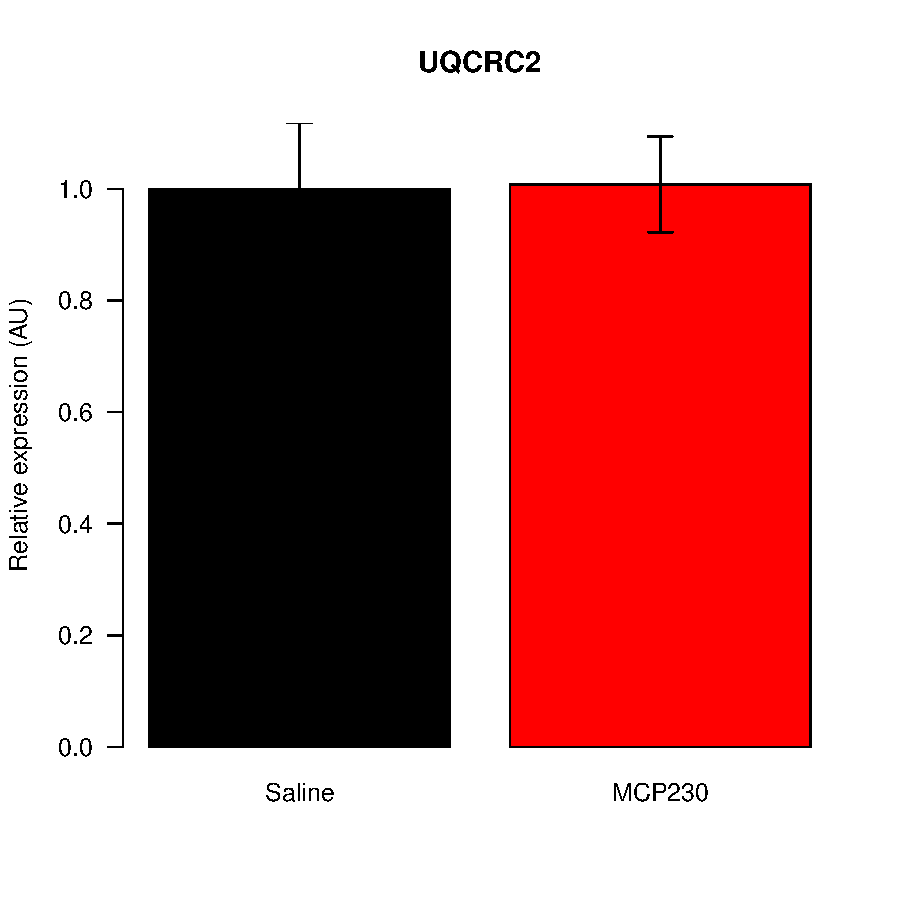
\includegraphics{2016-01-21_MitochondrialProteins-barplotUQCRC2}
\end{center}
\caption{Barplot of Relative UQCRC2 Protein Expression in Quadriceps Muscle, Saline versus MPI}
\label{fig:barplotUQCRC2}
\end{figure}

\begin{figure}
\begin{center}
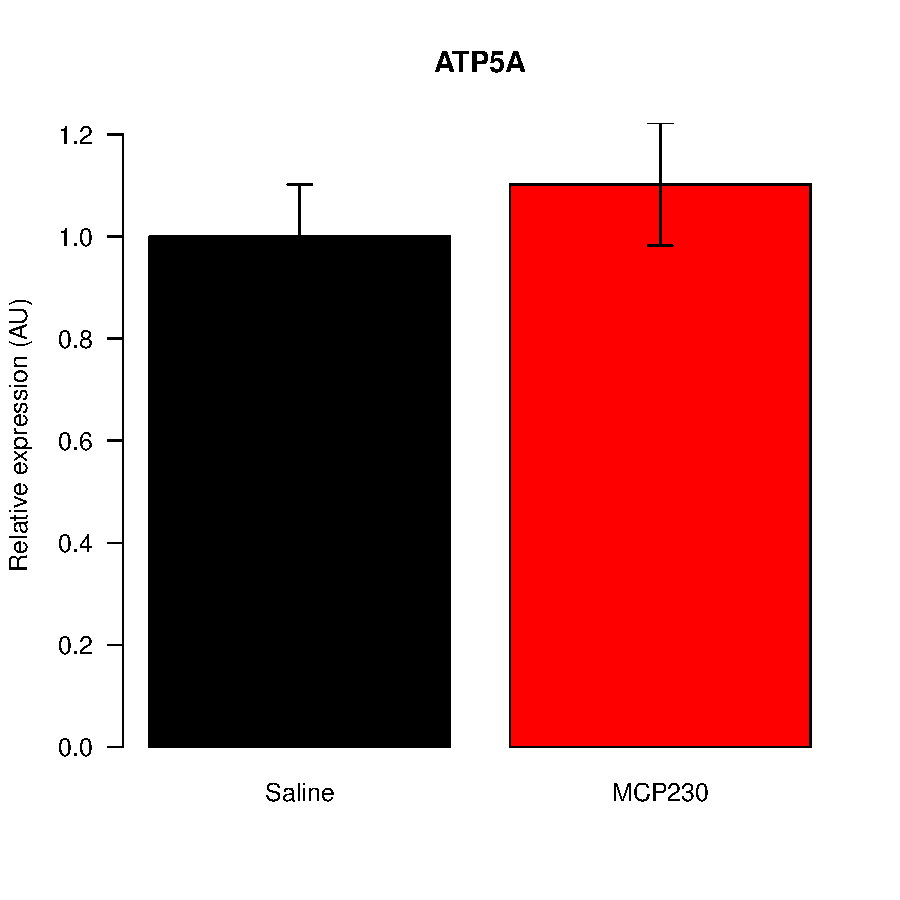
\includegraphics{2016-01-21_MitochondrialProteins-barplotATP5A}
\end{center}
\caption{Barplot of Relative ATP5A Protein Expression in Quadriceps Muscle, Saline versus MPI}
\label{fig:barplotATP5A}
\end{figure}

\begin{figure}
\begin{center}
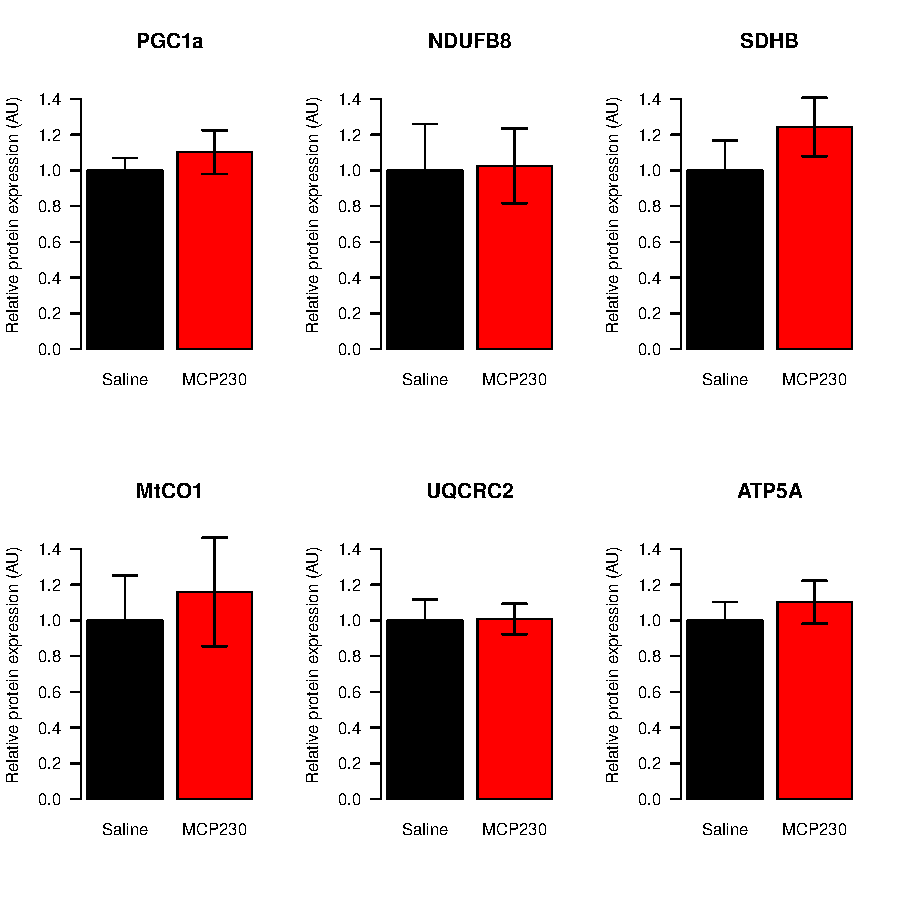
\includegraphics{2016-01-21_MitochondrialProteins-barplot-combined}
\end{center}
\caption{Barplot of the OXPHOS proteins}
\label{fig:barplot-combined}
\end{figure}

\section*{Session Information}
\begin{itemize}\raggedright
  \item R version 3.1.1 (2014-07-10), \verb|x86_64-w64-mingw32|
  \item Locale: \verb|LC_COLLATE=English_United States.1252|, \verb|LC_CTYPE=English_United States.1252|, \verb|LC_MONETARY=English_United States.1252|, \verb|LC_NUMERIC=C|, \verb|LC_TIME=English_United States.1252|
  \item Base packages: base, datasets, graphics, grDevices, methods,
    stats, utils
  \item Other packages: car~2.0-25, plyr~1.8.3, rJava~0.9-7,
    xlsx~0.5.7, xlsxjars~0.6.1
  \item Loaded via a namespace (and not attached): grid~3.1.1,
    lattice~0.20-29, lme4~1.1-10, MASS~7.3-33, Matrix~1.2-3,
    MatrixModels~0.4-1, mgcv~1.8-0, minqa~1.2.4, nlme~3.1-117,
    nloptr~1.0.4, nnet~7.3-8, parallel~3.1.1, pbkrtest~0.4-4,
    quantreg~5.19, Rcpp~0.12.2, SparseM~1.7, splines~3.1.1, tools~3.1.1
\end{itemize}

\end{document}
